\documentclass[12pt]{article}

% ========== Paquetes ===========

% Codificación de caracteres e idioma
\usepackage[utf8]{inputenc}
\usepackage[spanish]{babel}

% Tamaño de página y márgenes
\usepackage[letterpaper, margin=2.54cm]{geometry}

% Comillas, columnas, gráficos, símbolos matemáticos e ingreso de código de programación
\usepackage{csquotes, multicol, graphicx, amssymb, amsmath, listings, xcolor}

% Uso de imágenes SVG
\usepackage{svg}

% Interlineado 1.5
\usepackage{setspace}
\onehalfspacing

% Separación de columnas y sangría
\setlength{\columnsep}{2cm} 
\setlength{\parindent}{0cm}

% Páginado
\pagestyle{plain}

% Evitar separación de palabras
\hyphenpenalty=10000
\exhyphenpenalty=10000
\sloppy

% ========== Documento ==========

\begin{document}

% ========== Portada ============
\begin{titlepage}
	\centering
	{\scshape\LARGE Universidad Aztlán \par}
	\vspace{1cm}
	{\scshape\Large Campus Playa del Carmen \par}
	\vspace{1.75cm}
	{\scshape\Huge  Diagramas de Modelo Entidad-Relación \par}
    \vfill
    {\itshape\Large Con notación de Peter Chen \par}
	\vspace{2cm}
    {\itshape\Large Presentado por: \par}
	{\Large José Rosendo Camal Teh \par}
	\vfill
	{\Large Ingeniería en Sistemas Computacionales \par}
	{\Large Cuarto Cuatrimestre \par}
	{\Large Fundamentos de Bases de Datos \par}
	\vfill
	{\Large Profe. Emmanuel Andrés Martínez López \par}
	\vfill
	{\Large 11 de octubre de 2026 \par}
	\vfill
	{\Large Playa del Carmen, Quintana Roo \par}
\end{titlepage}
\newpage

\listoffigures
\newpage

\section*{\centering Diagramas MER}
\addcontentsline{toc}{section}{Diagramas MER}

\begin{figure}[htb]
	\centering
	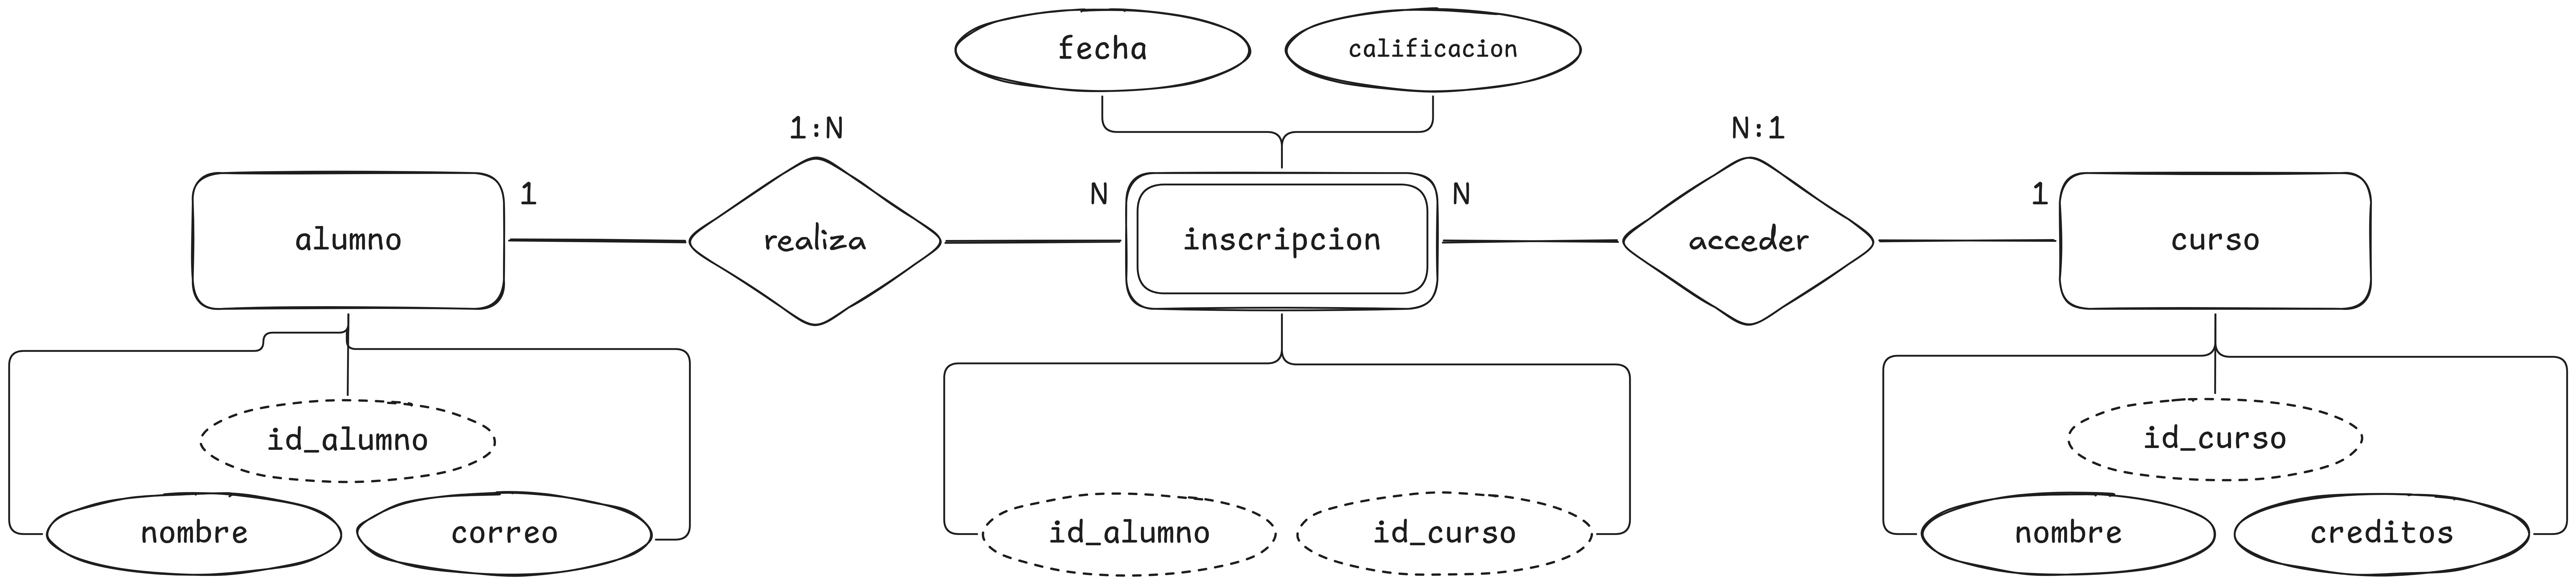
\includegraphics[width=1\textwidth]{img/asignaciones.excalidraw.png}
	\caption{Asignaciones}
    \label{fig:asignaciones}
\end{figure}

En la \textbf{Figura \ref{fig:asignaciones}} se muestra las relaciones ulteriores:
\begin{itemize}
    \item La relación entre las entidades \texttt{alumno} e \texttt{inscripcion} es del tipo \textbf{1:N}. Esto se debe a que un \textit{alumno} puede realizar varias inscripciones (solicitudes para cursar alguna asignatura), pero una \textit{inscripción} solo puede tener relación con un único alumno.
    \item La relación entre las entidades \texttt{inscripcion} y \texttt{curso} es de cardinalidad \textbf{N:1}. Este tipo de relación se debe a que una \textit{inscripción} puede tener vínculo con un único curso, pero un \textit{curso} puede estar en varias solicitudes de inscripción.
\end{itemize}

\begin{figure}[htb]
	\centering
	
\includegraphics[width=1\textwidth]{img/libreria.excalidraw.png}
	\caption{Librería \textquote{El Párrafo}}
    \label{fig:libreria}
\end{figure}

En la \textbf{Figura \ref{fig:libreria}} se muestra las relaciones ulteriores:
\begin{itemize}
    \item La relación \texttt{venta-cliente} es de tipo \textbf{N:1}. Esto es así porque cada \textit{venta} está relacionada con un único cliente, pero un \textit{cliente} puede ejecutar varias compras.
    \item La relación \texttt{cliente-libro} es de tipo \textbf{N:M}. Esto es así porque cada \textit{cliente} puede adquirir varios libros. De forma análoga, un \textit{libro} puede estar vinculado con varios clientes.
    \item La relación \texttt{libro-autor} es de tipo \textbf{N:M}. Esto es así porque cada \textit{autor} puede tener la autoría de uno o varios libros y un \textit{libro} puede estar escrito por varios autores.
\end{itemize}

\end{document}